\chapter{提案手法}
\thispagestyle{empty}
\label{chap2}
\minitoc

\newpage
%%%%%%%%%%%%%%%%%%%%%%%%%%%%%%%%%%%%%%%%%%%%%%%%%%%%%%%%%%%%%%%%%%%%%%%%%%%%%%%
%==============================================================================
%はじめに
%==============================================================================
\section{はじめに}
本章では,画像による3次元物体検出と点群位置合わせによるダンプトラックの位置姿勢推定をするための手法について述べる.
\par
2.2 節では,ダンプトラックの位置姿勢を推定するために画像による3次元物体と点群位置合わせを統合したダンプトラックの位置姿勢推定のアプローチについて述べる.
\par
2.3 節では,画像による3次元物体検出の手法について述べる.
\par
2.4 節では,点群位置合わせによるダンプトラックの位置姿勢推定について述べる.
\newpage

\section{位置姿勢推定のアプローチ}
\subsection{画像による3次元物体検出と点群位置合わせによる位置姿勢の概要}
第 1 章で述べたように本研究ではダンプトラックの位置姿勢を計測するために画像による3次元物体検出と点群位置合わせを統合した位置姿勢推定の手法を用いる.
その概要について説明する.
\par
事前に点群位置合わせの基準となるダンプトラックの3次元モデルを作成を行う.土砂積み込み作業範囲に
設置したダンプトラックを計測することで3次元点群を取得する.取得した3次元点群は地面情報やノイズを含むためダンプトラックの点群を抽出することで3次元モデルを作成する.
\par
次に位置姿勢推定の概要について説明する.
ダンプトラックは土砂積み込み作業範囲外からバックホウに向かって進入すると仮定する.遠方からバックホウに向かって進入するダンプトラックを
画像による3次元物体検出により大まか位置姿勢を計測する.また,推定値が土砂積み込み作業範囲外であれば範囲内に進入するまで3次元物体検出を行い,
範囲内であれば,推定値を初期値とした,点群位置合わせにより位置姿勢推定を行う.
点群位置合わせは基準モデルと計測データが必要だが,基準モデルには事前に作成したダンプトラックの3次元モデル,計測データにはバックホウに搭載した距離センサから計測した
3次元点群を用いる.
また,3次元物体検出の際,ダンプトラックが映っているのにかかわらず推定に失敗する場合ある.そのため,検出に失敗した場合は直前のフレームを参照し,ダンプトラックの位置が土砂積み込み
作業範囲内であれば3次元特徴量マッチングを初期値とした点群位置合わせにより位置姿勢推定を行う.
\newpage
\subsection{位置姿勢推定システムの概要}
本節では,画像による3次元物体検出や点群位置姿勢に必要となる画像や点群を計測する方法を説明する.
ダンプトラックのような大型車両を計測するにあたり,バックホウのキャビン上部から計測することでダンプトラックの全体を捉えることが可能となる.
しかし,ダンプトラックが大きく旋回した場合オクルージョンが発生し点群位置合わせに大きく誤差が生じる.そのため図に示すように複数台の距離画像センサを扇状に設置することで死角を減らす.
また,複数台の距離画像センサから計測した3次元点群を結合するには,各センサ間の位置姿勢が必要となる.本研究では各センサからArUcoボード\cite{Garrido2015}を
撮影することで各センサから見たArUcoボードの位置姿勢を計測,その位置姿勢を基に各センサの位置姿勢を導出する.
結合した3次元点群はカメラ座標系のためバックホウとダンプトラックの相対的な位置関係が把握できない.
そのためセンサに搭載したIMUにより地面と並行になるように座標変換を行う.
\newpage
\section{画像による3次元物体検出}
\subsection{深層学習による3次元物体検出}
本項では深層学習による3次元物体検出について述べる.本研究では単一の画像から求めたCNN特徴量から対象の中心距離$(C_x, C_y, C_z)$とカメラから見た姿勢$\theta$,
画像内の領域を推定する3D Bounding Box Estimation Using Deep Learningand Geometry\cite{2017}を用いる.
この手法においては,図\ref{fig:pose}に示すように入力画像から画像内の領域を推定後,対象物体のローカル座標系の回転 $\theta_l$と中心の距離$(C_x, C_y, C_y)$の推定を行うことで対象物体の位置姿勢を求める.

以下の式でカメラの内部パラメータ$R$により対象物体の距離から画像座標$(u, v)$に変換を行う.
\begin{equation}
\begin{bmatrix}u  \\v \\1 \end{bmatrix}
=\begin{bmatrix}f_x & 0 & c_x\\0 & f_y & c_y\\0 &0 &1 \end{bmatrix}
\begin{bmatrix}\frac{x}{z}  \\\frac{y}{z} \\1 \end{bmatrix}
\end{equation}


図\ref{fig:ray}に示すように,対象物体の画像座標$(u, v)$とカメラの画像中心$(c_x, c_y)$のなす角$\theta_{ray}$を求め以下の式で対象物体の姿勢を算出する.


\begin{equation}
    \theta =
     \theta_l-\theta_{ray}
 \end{equation}
また,この手法は一般車両の自動運転を目的としたものであり,図\ref{fig:kitti}に示すように自動運転用のデータセットであるKITTIデータにを基に学習を行うため,ダンプトラックのような建設機械は
データ数がないため認識精度は低いという問題がある.
\clearpage

\begin{figure}[b]
    \begin{center}
    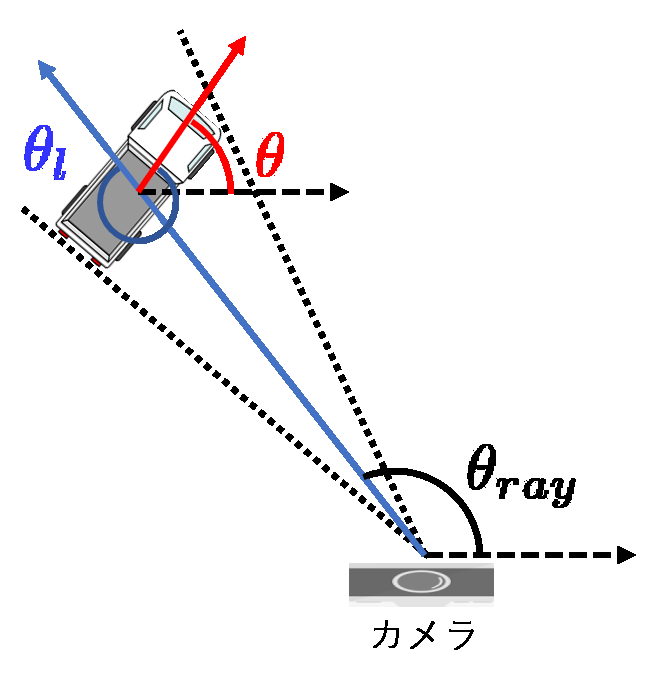
\includegraphics[width=0.5\columnwidth]{./chap2/fig/3DBox.eps}
    \caption{姿勢の導出方法}
    \label{fig:pose}
    \end{center}
    %\vspace{-5mm}
\end{figure}


\begin{figure}[b]
    \begin{center}
    \includegraphics[width=0.8\columnwidth]{./chap2/fig/ray.eps}
    \caption{物体中心と画像中心のなす角の導出}
    \label{fig:ray}
    \end{center}
    %\vspace{-5mm}
\end{figure}

\begin{figure}[b]
    \begin{center}
    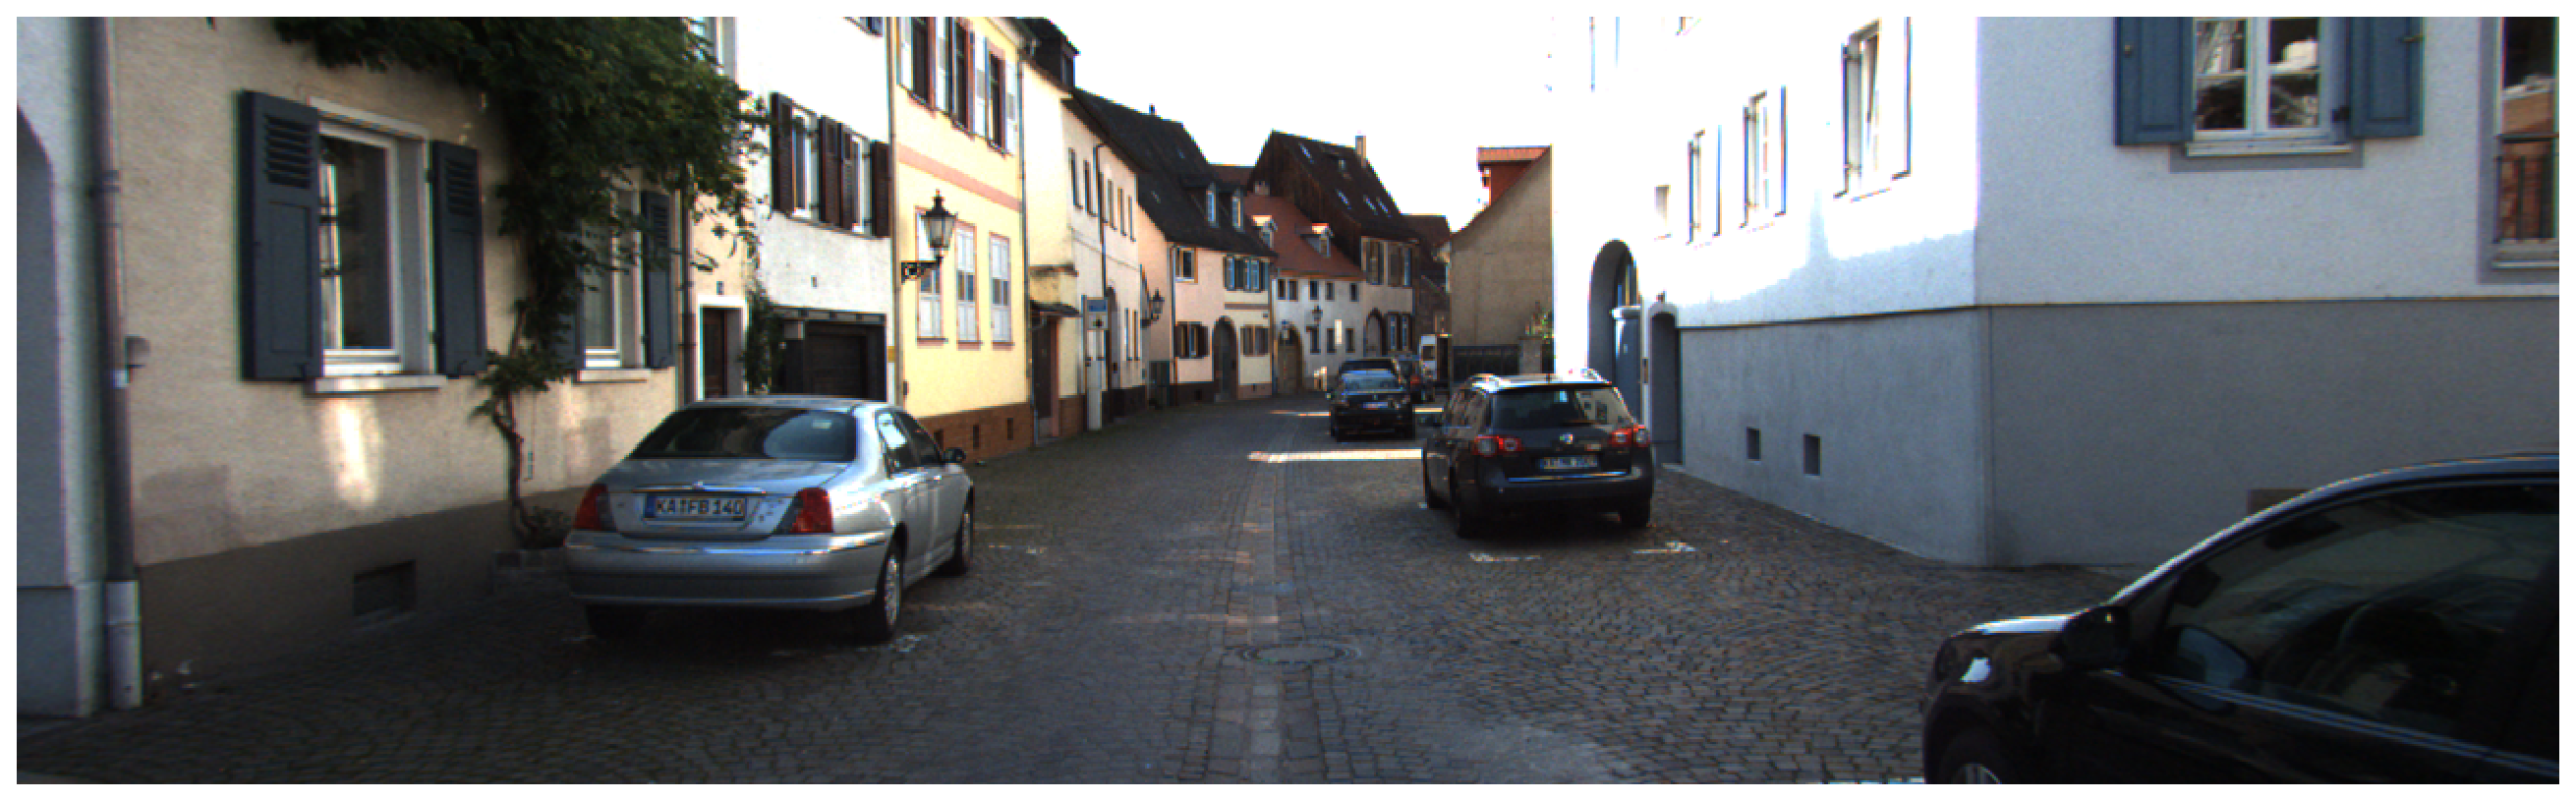
\includegraphics[width=0.8\columnwidth]{./chap2/fig/kitti.eps}
    \caption{KITTIデータセット}
    \label{fig:kitti}
    \end{center}
    %\vspace{-5mm}
\end{figure}


\clearpage

\subsection{データセットの作成}
本項では深層学習による3次元物体検出によりダンプトラックを認識するために必要な学習用データセットの作成方法について述べる.
2.3.1 節で述べたように,深層学習による3次元物体検出は一般車両の自動運転を目的としたものであるため,ダンプトラックのような建設機械は
データ数が少ないため認識精度は低い.そのため本研究では,認識精度向上させるためにダンプトラックの模型を用いた学習用のデータセット作成を行う.
データセットを作成するためにはダンプトラックの画像,中心位置$(C_x, C_y, C_z)$,ローカル座標系の姿勢$\theta_l$,寸法と対象物体の画像座標が必要となる.そのため,図\ref{fig:train}に示すように,撮影環境を構築する.
回転台の上にダンプトラックを設置することで回転台から$\theta_c$を計測し,RGB-Dカメラにより画像と位置を獲得する.その後,撮影した画像からダンプトラックの画像座標を
ラベル付することでデータセットの作成を行う.
また,データセットを拡張するために背景をクロマキー合成を行う.


%%%%%
\begin{figure}[b]
    \begin{center}
    \includegraphics[width=0.8\columnwidth]{./chap2/fig/training.eps}
    \caption{撮影環境}
    \label{fig:train}
    \end{center}
    %\vspace{-5mm}
\end{figure}
%%%%
\newpage

\section{点群位置合わせによる位置姿勢推定}
\subsection{ダンプトラックの点群抽出}
本項では距離センサから計測した点群から点群位置合わせの基準となるダンプトラックの点群を抽出する方法を述べる.
計測した点群は、イズや土砂積み込み作業範囲外の点群などの不要な点群が含まれるためフィルタリングする.まず,土砂積み込み作業範囲を超える点群を除去する,この作業範囲は現場ごとに既知である.さらに
地面の点群は位置合わせに不要であるため,RANSAC (RANdom SAmple Consensus)\cite{Fischler1981}による平面検出を用いることで,ダンプトラックと地面に分割し,除去する.その後,得られた点群の各点に対して,
近傍点までの距離を基準に外れ値を除去するStatistical Outlier Removalフィルタを用いることで,ダンプトラック以外のノイズを除去する,この際,計算量を削減しオンサイトでの推定を実現するために,
位置姿勢推定の基準となる点群だけに適用する.不要な点群を除去後,
点群をボクセルに変換することで平滑化し,ダンプトラックにのっている微細なノイズを減らす.
\newpage

\subsection{点群位置合わせ}
本項では点群位置合わせによるダンプトラックの位置姿勢の推定手法ついて述べる.
本研究ではICP(Iterative ClosestPoint)\cite{Chetverikov2002}により点群位置合わせを行う.
ICPにおいては,図\ref{fig:icp}に示すように,基準点群と計測点群の近傍点を対応点として扱い,対応点間のユーグリッド距離を
最小2乗法により最小化を繰り返し,高精度な位置合わせをすることで回転と移動量を導出し位置姿勢推定を行う.
\begin{figure}[b]
    \begin{center}
    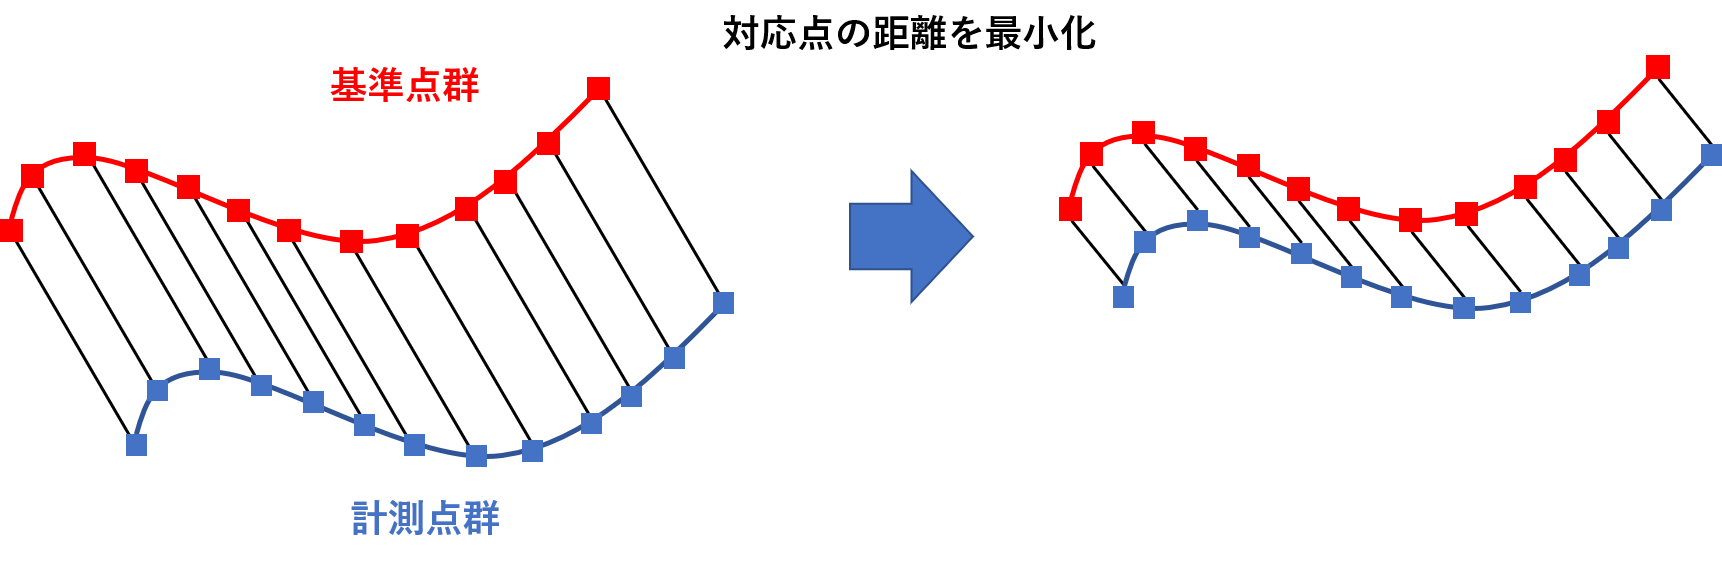
\includegraphics[width=1.0\columnwidth]{./chap2/fig/ICP.eps}
    \caption{ICP アルゴリズム}
    \label{fig:icp}
    \end{center}
    %\vspace{-5mm}
\end{figure}


\newpage

\subsection{3次元特徴量マッチング}
本項では点群位置合わせの初期値となる3次元特徴量マッチングについて述べる.
本研究では,FPFH(Fast PointFeature Histogram)\cite{Rusu2009}により対応点の検出を行う.
FPFHにおいては,各点と近傍点との法線の関係の分布ををヒストグラム化した特徴量であり,外乱に頑健かつ回転にも強いという利点を持つ.
FPFHにより対応点を検出行い,対応点を基にパラメータ推定することで移動量と回転量を求めるが,外れる値が含まれると大きな誤差が発生する.
そのため,RANSACアルゴリズムを用いることで外れる値にロバストなパラメータ推定を行う.

\newpage

\section{おわりに}
本章では,画像による3次元物体検出と点群位置合わせによるダンプトラックの位置姿勢推定の手法について述べた.
\par
2.2 節では,画像による3次元物体検出と点群位置合わせを統合するための本研究のアプローチ
について述べた.
\par
2.3 節では,画像による3次元物体検出手法について述べた.
2.4 節では,点群位置合わせによる位置姿勢推定の手法について述べた.

\newpage